\section{Overview of game theoretic model} \label{sec:model_overview}

The problem studied is a 3-player normal form game. The players are:
  
\begin{itemize}
    \item the decision makers of two queueing systems;
    \item a service that distributes individuals to these two queueing systems.
\end{itemize}

This is a standard Normal form game~\cite{Maschler2013},  
in that each player in this game has their own objectives which they aim to 
optimise.
More specifically, the queueing systems' objective is captured by an upper bound
of the time that a fixed proportion of individuals spend in the system, 
while the distributor aims to minimise the time that its individuals 
are blocked.
% TODO: Depending on how this is described earlier, we might need a little more 
% here (as to what we mean by "blocked")

The queueing systems are designed in such a way where they can accept two types
of individuals. 
These are the individuals that the distributor allocates to them and 
other individuals from other sources. 
Each queueing system may then choose to block the individuals that arrive from 
the distributor when the system reaches a certain capacity. 
The strategy sets for each queueing system is the set 
\( \{T \in \mathbb{N} \;|\; 1 \leq T \leq N\} \) where \(N \in\{N_A, N_B\}\) are 
the total capacities of the two queueing systems. We denote the chosen actions 
from the strategy set as \(T_A, T_B\) and call these \textit{threshold}s.

Both queueing systems follow a queueing model that has two waiting spaces for 
individuals. 
The first waiting zone is where the individuals queue right before receiving 
their service and has a capacity of \( N - C \), where \(N\) is the total 
capacity of the waiting space and \(C\) is the number of servers. 
The second waiting zone is where the individuals, that are sent from the 
distributor, stay until they are allowed to enter the first waiting zone.
The second waiting zone has a capacity of \(M\) and no servers.

This is shown diagrammatically in Figure ~\ref{fig:diagram_of_queueing_system}.

\begin{figure}[h]
    \centering
    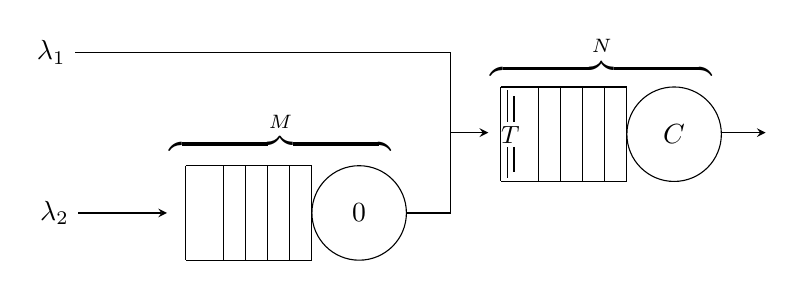
\begin{tikzpicture}[>=stealth, scale=0.8],
        % the rectangle of Queue 1
        \draw (0,0) -- ++(2cm,0) -- ++(0,-1.5cm) -- ++(-2cm,0);
        % The label above Queue 1 -> M
        \node[anchor=north] at (1.5cm, 1cm) {\( 
            \overbrace{\qquad \qquad \qquad \qquad}^{M} 
        \)};
        % the vertical lines in Queue 1
        \foreach \i in {1,...,4, 5.7}
        \draw (2cm-\i*10pt,0) -- +(0,-1.5cm);
        
        % the circle in Queue 1
        \draw (2.75,-0.75cm) circle [radius=0.75cm] node {\(0\)};

        % the rectangle in Queue 2
        \draw (5,1.25) -- ++(2cm,0) -- ++(0,-1.5cm) -- ++(-2cm,0);
        % the vertical lines in Queue 2
        \foreach \i in {1,...,4, 5.7}
        \draw (7cm-\i*10pt,1.25) -- +(0,-1.5cm);
        % The two vertical lines at the very start of Queue 2 
        \draw (7cm-54pt,1.2) -- +(0,-0.5cm);
        \draw (7cm-54pt,0.3) -- +(0,-0.5cm);        
        \draw (7cm-51pt,1.1) -- +(0,-0.4cm);
        \draw (7cm-51pt,0.3) -- +(0,-0.4cm);

        % The label between the lines for T
        \node[anchor=north] at (5.15, 0.77 cm) {\small{\( T \)}};

        % The label above Queue 2 -> N
        \node[anchor=north] at (6.6cm, 2.2cm) {\( 
            \overbrace{\qquad \qquad \qquad \qquad}^{N} 
        \)};

        % the circle in Queue 2
        \draw (7.75,0.5) circle [radius=0.75cm] node {\(C\)};

        % Arrow line from Queue 2 outside
        \draw[->] (8.5,0.525) -- +(20pt,0);
        
        % Line from lambda_2 to Queue 1
        \draw[<-] (-0.3,-0.75) -- +(-40pt,0) node[left] {\( \lambda_2 \)};
        % First line (horizontal) after Queue 1
        \draw[-] (3.5,-0.75) -- +(20pt,0);
        % Second line (vertical) after Queue 1
        \draw (4.2, 0.525) -- (4.2, -0.75);
        
        % First line (horizontal) from lambda_1
        \draw (4.2, 1.8) -- +(-169.5pt,0) node[left] {\( \lambda_1 \)};
        % Second line (vertical) from lambda_1
        \draw (4.2, 1.8) -- (4.2, 0.525);
        % Arrow line to Queue 2
        \draw[->] (4.2, 0.525) -- (4.8, 0.525);  
    \end{tikzpicture}
    \caption{A diagrammatic representation of the queueing model. 
    The threshold \(T\) only applies to arrivals from the first buffer. 
    If the second buffer is at that threshold only individuals of the first type 
    are accepted (at a rate \(\lambda_1\)) and individuals of the second type 
    (arriving at a rate \(\lambda_2\)) are held blocked in the first buffer.}
    \label{fig:diagram_of_queueing_system}
\end{figure}

Note here that both types of individuals can become lost to the system. 
Individual allocated from the distributor become lost to the system whenever 
an arrival occurs and the second waiting zone is at full capacity (\(M\) 
individuals already waiting).
Similarly, other individuals get lost whenever they arrive at the first waiting 
zone and it is at full capacity (\(N - C\) individuals already waiting).

Following this queuing model, the two queueing systems' choice of strategy will 
then rely solely on satisfying their own 
objective, which is to make sure that the waiting time in the first waiting zone 
of a proportion of individuals will be below the predefined target time.

\begin{equation}
    P(W < R) \geq \hat{P}
\end{equation}

where \(W\) is the mean waiting time of all individuals, \(R\) is the time 
target and \(\hat{P}\) is the percentage of individuals need to be within that 
target. 
There are numerous objective functions that can be used to capture this 
behaviour. 
For example one approach is to use the threshold that maximises the probability 
that 
the mean waiting is more than the target time, and completely ignore the 
percentage goal.

\begin{equation}
    \arg \max_{T_i} \quad P(W_i < R)
\end{equation}

A more sophisticated objective function would be to get the proportion 
of individuals as close to the percentage aim. 
In other words, to find the threshold that minimises the difference between the 
probability and the percentage goal (or maximise its negation).

\begin{equation}\label{eq:obj-queueing-systems}
    \arg \max_{T_i} \quad -\left( \hat{P} - P(W_i < R) \right)^2
\end{equation}


The third player, the distributor has their own choices to make and their own 
goals to satisfy.
The strategy set of the third player is the proportion \(0 \leq p \leq 1\) of 
individuals it sends to the first queueing system (the proportion \(1 - q\) is 
sent to the second queueing system).
In addition, the distributor aims to minimise any potential blockages
that may occur, given the pair of thresholds chosen by the two queueing systems.
Thus, its objective is to minimise the blocked time of the individuals 
that they send to the two queueing systems.
Apart from the time being blocked, an additional aspect that may affect the 
decision of the distributor is the proportion of lost individuals.
Equation \ref{eq:obj-distributor} can be used to capture a mixture 
between the two objectives.

\begin{equation}\label{eq:obj-distributor}
    \alpha P(L_A) + (1 - \alpha) B_A = 
    \alpha P(L_B) + (1 - \alpha) B_B
\end{equation}

Here, \(\alpha\) represents the ``importance'' of each objective,
where high \(\alpha\) indicates a higher weight on the proportion of lost 
individuals and smaller \(\alpha\) a higher weight on the time blocked. 


Using equations \ref{eq:obj-queueing-systems} and \ref{eq:obj-distributor} gives
an imperfect information extensive form game. 
An imperfect information game is defined as an extensive form game where some 
of the information about the game state is hidden for at least one of the 
players~\cite{Berwanger2008}. In this study the state of the problem that is
hidden is the threshold that each of the first two players chooses to play.
In other words, each queueing system chooses to play a strategy without the 
knowing the other system's strategy.
The distributor then, fully aware of the chosen threshold strategies, distributes 
individuals among the two systems in order to minimise the time that its 
individuals will be blocked. Figure \ref{fig:imperfect-info-game} illustrates this. 

\begin{figure}[ht]
    \centering
    \begin{tikzpicture}[-, node distance = 3cm, scale=0.8]
        \node[anchor=north](HA){\(H_A\)};
        \node[anchor=north](HA_d1) at (3, 2){.};
        \node[anchor=north](HA_d2) at (3, -2){.};
    
        \path[->] (HA) edge node {}(HA_d1);
        \path[->] (HA) edge node {}(HA_d2);
        \path (HA_d1) edge [bend left] node {}(HA_d2);
        \path (HA_d1) [dashed] edge node {}(HA_d2);
    
        \node[anchor=north](HB) at (4.1, 0){\(H_B\)};
        \node[anchor=north](HB_d1) at (6.9, 2){.};
        \node[anchor=north](HB_d2) at (6.9, -2){.};
    
        \path[->] (HB) edge node {}(HB_d1);
        \path[->] (HB) edge node {}(HB_d2);
        \path(HB_d1) edge [bend left] node {}(HB_d2);
    
        \node[anchor=north](D) at (7.8, 0){\(D\)};
        \node[anchor=north](D_d1) at (10.8, 2){.};
        \node[anchor=north](D_d2) at (10.8, -2){.};
        
        \path[->] (D) edge node {}(D_d1);
        \path[->] (D) edge node {}(D_d2);
        \path(D_d1) edge [bend left] node {}(D_d2);
    \end{tikzpicture}
    \caption{Imperfect information Extensive Form Game between the distributor 
    and the 2 queueing systems}
    \label{fig:imperfect-info-game}
\end{figure}

The first 
queueing system \(H_A\) decides on a threshold, then the second system \(H_B\)
chooses its own threshold, without knowing the strategy of \(H_A\), and finally
the distributor makes its choice. Note here that the dotted line represents the
fact that \(H_B\) is unaware of the state of the game when making its own 
decisions. The game can thus be partitioned into a normal form game between the
two queueing systems and finding the distributor's best choice. 

In order to define the normal form game the two payoff matrices of the players 
are required. From equation \ref{eq:obj-queueing-systems} the utilities of the
players can be formulated as:

\begin{equation}
    U_{T_1, T_2}^i = \quad -\left( 
        \hat{P} - P(W_i < R) 
    \right)^2
\end{equation}

Consequently, the payoff matrices of the game can be populated by these 
utilities:

\begin{equation} \label{eq:payoff-matrices}
    A = 
    \begin{pmatrix}
        U_{1,1}^A & U_{1,2}^A & \dots & U_{1,N_B}^A \\
        U_{2,1}^A & U_{2,2}^A & \dots & U_{2,N_B}^A \\
        \vdots & \vdots & \ddots & \vdots \\
        U_{N_A,1}^A & U_{N_A,2}^A & \dots & U_{N_A,N_B}^A \\
    \end{pmatrix},
    B = 
    \begin{pmatrix}
        U_{1,1}^B & U_{1,2}^B & \dots & U_{1,N_B}^B \\
        U_{2,1}^B & U_{2,2}^B & \dots & U_{2,N_B}^B \\
        \vdots & \vdots & \ddots & \vdots \\
        U_{N_A,1}^B & U_{N_A,2}^B & \dots & U_{N_A,N_B}^B \\
    \end{pmatrix}
\end{equation}

Based on the choice of strategy of these two players the distributor will then 
make their own choice of the proportion of individuals to send to each system.
